% Copyright (C) 2026 Joshua Macdonald
% SPDX-License-Identifier: GPL-3.0-or-later
\documentclass[tikz,border=9pt]{standalone}
\usepackage[T1]{fontenc}
\usepackage{lmodern}
\usetikzlibrary{arrows.meta}
\renewcommand{\familydefault}{\sfdefault}
\definecolor{Ink}{HTML}{263D4A}
\definecolor{Blue}{HTML}{24678E}
\definecolor{Teal}{HTML}{0D6B6E}
\definecolor{Gold}{HTML}{87641A}
\pdfinfoomitdate=1
\pdftrailerid{}
\pdfsuppressptexinfo=15
\tikzset{every node/.style={font=\sffamily\fontsize{11}{14}\selectfont,text=Ink},
  panel/.style={draw=#1!65,fill=#1!5,rounded corners=4pt,
    minimum width=3.8cm,minimum height=2.7cm,text width=3.1cm,
    inner sep=8pt,align=left,anchor=north west},
  flow/.style={-{Stealth},draw=Ink,shorten <=3pt,shorten >=3pt}}
\begin{document}
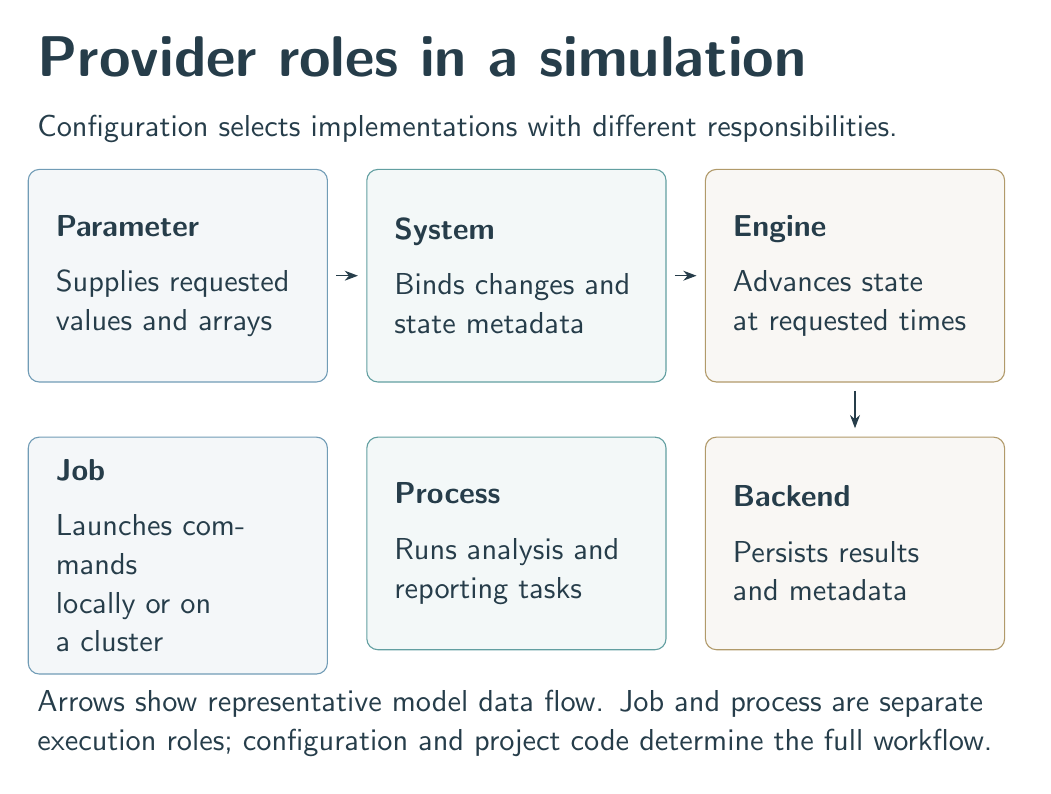
\begin{tikzpicture}
\node[anchor=north west,font=\sffamily\bfseries\fontsize{21}{25}\selectfont] at (0,1.8) {Provider roles in a simulation};
\node[anchor=north west,text width=12.4cm] at (0,.8) {Configuration selects implementations with different responsibilities.};
\node[panel=Blue] (parameter) at (0,0) {\textbf{Parameter}\\[6pt]Supplies requested\\values and arrays};
\node[panel=Teal] (system) at (4.3,0) {\textbf{System}\\[6pt]Binds changes and\\state metadata};
\node[panel=Gold] (engine) at (8.6,0) {\textbf{Engine}\\[6pt]Advances state\\at requested times};
\node[panel=Blue] at (0,-3.4) {\textbf{Job}\\[6pt]Launches commands\\locally or on\\a cluster};
\node[panel=Teal] at (4.3,-3.4) {\textbf{Process}\\[6pt]Runs analysis and\\reporting tasks};
\node[panel=Gold] (backend) at (8.6,-3.4) {\textbf{Backend}\\[6pt]Persists results\\and metadata};
\draw[flow] (parameter.east) -- (system.west);
\draw[flow] (system.east) -- (engine.west);
\draw[flow] (engine.south) -- (backend.north);
\node[anchor=north west,text width=12.4cm] at (0,-6.5) {Arrows show representative model data flow. Job and process are separate execution roles; configuration and project code determine the full workflow.};
\end{tikzpicture}
\end{document}
